% ACL format when acl.sty is available; otherwise a plain two-column fallback.
\IfFileExists{acl.sty}{%
  \documentclass[11pt]{article}%
  \usepackage[final]{acl}%
}{%
  \documentclass[11pt,twocolumn]{article}%
  \usepackage[letterpaper,margin=1in]{geometry}%
  \usepackage[round,authoryear]{natbib}%
  \setlength{\columnsep}{0.25in}%
}
\usepackage{times}
\usepackage{latexsym}
\usepackage[T1]{fontenc}
\usepackage[utf8]{inputenc}
\usepackage{microtype}
\usepackage{graphicx}
\usepackage{booktabs}
\usepackage{tabularx}
\usepackage{amsmath}
\usepackage{url}
\usepackage{listings}
\lstdefinestyle{prompt}{basicstyle=\ttfamily\fontsize{6.6pt}{7.3pt}\selectfont,
  breaklines=true,breakatwhitespace=false,columns=fullflexible,
  keepspaces=true,frame=single,xleftmargin=0pt}
\usepackage{tikz}
\usetikzlibrary{arrows.meta,positioning,shapes.geometric,calc}

\title{DFM at DocSEM 2026: Investigating a Guided-Reasoning Pipeline\\
for Open Models Under a Validation--Test Shift}

\author{%
  Dyonnatan Ferreira Maia \\
  \texttt{dyonnatan@egresso.ufg.br}
}

\date{}

\begin{document}
\maketitle

\begin{abstract}
Can frozen open-weight models solve document-grounded mathematics better
with inference-time guidance alone? We study DocSEM, where systems answer a
quantitative query and cite its supporting block. Our training-free pipeline
generates rival readings, evaluates their arithmetic in code, and filters them
with validators and fixed rules. It achieves 88.5\% answer accuracy on
validation but 51.4\% on test. The test split differs: each document contains
about two dozen problems and lexical decoys, so the model must first select the
relevant passage. On a synthetic test-like replica matching our first test
answer accuracy within three points, selection errors are about seven times as
frequent as resolution errors (wrong answers from the right passage).
Accordingly, resolution-focused guidance adds little; a step-level DSL does not
improve accuracy over rival readings, although it provides a structured,
inspectable trace. The largest gain comes from a short post-competition
selection instruction: with it, the pipeline raises replica answer accuracy
over direct prompting from 46.3\% to 68.3\% (DeepSeek-V4-Flash) and from
64.4\% to 77.7\% (GLM-5.3-Flash). In an exploratory comparison, the best guided
open model reaches 67.0\% joint accuracy on the replica, against 82.0\% for a
closed coding agent; our ranked submission reached 45.09\%, against 85.09\% for
the best entry.
\end{abstract}

\section{Introduction}
\label{sec:intro}

DocSEM (DocInsights 2026, Task 1) asks a system to read a rendered PDF, find
the quantitative passage a paraphrased query refers to, and return the numeric
answer with the identifier of the supporting block. The problems are semantic variants \citep{singh2026gsmsem} of grade-school math word problems \citep{cobbe2021gsm8k}. The ranking metric, joint
exact accuracy, requires both the answer and the evidence to be exactly right.

Open-weight models are cheaper to run and easier to inspect than closed ones,
but they are usually evaluated as they are, with one prompt and one answer.
Strong results on such tasks usually come from closed models, which cost API
budget and can change or be retired, or from open models adapted by
reinforcement learning \citep{deepseek2025r1}, fine-tuning or adapters
\citep{hu2022lora}, which require GPUs and labelled data. We study a third route. We keep open models frozen and change only
what surrounds the model call. We change what the model is asked to write, we
move the arithmetic into code, and we let deterministic rules decide between
the model's alternatives. Our research question is whether frozen open-weight
models can solve document-grounded mathematics better with this inference-time
guidance alone. A side effect is that the output becomes a short
derivation that a person can read, although we do not evaluate readability
here.

The system has two stages. Stage~1 converts each rendered page to text and is
held fixed (\S\ref{sec:extraction}). Stage~2 produces the answer and is the subject of the paper (\S\ref{sec:ladder}). We evaluate it on five sets
(\S\ref{sec:data}). A hard training subset, a 200-task development corpus and
the validation portal form the \emph{exploration} phase. A synthetic replica of
the more complex held-out test split and the test portal form the
\emph{test-regime} phase.

Our contributions are:
\begin{enumerate}
\item A training-free incremental ablation, \textsc{A0}$\rightarrow$\textsc{C2}$\rightarrow$%
      \textsc{C3}$\rightarrow$\textsc{C3C}: each variant changes one design
      decision and is compared with the previous one by paired exact tests,
      which shows which parts of the structure account for the gain.
\item A diagnosis of why gains from the exploration phase did not transfer
      to the test split, whose documents pose about two dozen problems instead
      of one. On a test-like replica that matches our first test answer accuracy
      within three points, choosing the wrong passage accounts for about seven
      times more error than getting the number wrong on the right passage.
\item Two exploratory analyses: a comparison with a closed coding agent, and
      the observation that, in our setting, instances of the same model did not catch each
      other's errors.
\end{enumerate}

Code and the replica generator are available at
\url{https://github.com/Dyonnatan/docsem-2026}.

\section{Task and evaluation sets}
\label{sec:data}

Answers are compared by normalised exact match, which ignores whitespace,
case, a leading final-answer marker and equivalent decimal forms. Evidence is
compared by exact set match against the gold block list, which in training
always holds one block. On the replica we count evidence as correct only when
it is exactly the target block.

\begin{table}[t]
\centering
\small
\setlength{\tabcolsep}{3pt}
\begin{tabularx}{\columnwidth}{llrl>{\raggedright\arraybackslash}X}
\toprule
set & source & $n$ & gold & role \\
\midrule
\multicolumn{5}{l}{\emph{exploration phase}} \\
hard-18   & train & 18   & public & recovering baseline failures \\
dev200    & train & 200  & public & regression corpus \\
val       & val   & 217  & portal & official check \\
\midrule
\multicolumn{5}{l}{\emph{test-regime phase}} \\
replica   & train & 300  & by constr. & test-like, labelled \\
test      & test  & 1730 & portal & final ranking \\
\bottomrule
\end{tabularx}
\caption{The five evaluation sets. The 908 training tasks are the pool for the
first two and for the replica. No model is trained on any of them.}
\label{tab:sets}
\end{table}

We use no training, so the 908 training tasks serve as a pool for analysis.
Table~\ref{tab:sets} lists the five sets drawn from it and from the official
splits. The \textbf{hard-18} set holds 16 dev200 tasks that direct prompting
and \textsc{C2}, both with DeepSeek-V4-Flash, and \textsc{C2} with a closed
model (GPT-5.6 Sol; \citealp{openai2026gpt56}) all missed. It adds two dev200 tasks that we used as
diagnostic cases for the validators. It is therefore a subset of dev200,
selected by failure, and we used it to explore models and technique
combinations. The \textbf{dev200} set holds 200 training tasks with public
answers and evidence and serves as the regression corpus. The \textbf{val} and
\textbf{test} splits are scored only by the official portal.

\begin{table}[t]
\centering
\small
\setlength{\tabcolsep}{4pt}
\begin{tabular}{lrr}
\toprule
per document & train / val & test \\
\midrule
characters                     & $\sim$5k & $\sim$43k \\
quantitative problems          & 1 & 23.6 \\
decoys repeating the query     & no & yes \\
block identifiers              & \texttt{bNN} & opaque \\
\bottomrule
\end{tabular}
\caption{Documents of the exploration splits and of the test split.}
\label{tab:shift}
\end{table}

The splits differ in one important respect (Table~\ref{tab:shift}). A train or val document is about
5k characters long and poses one quantitative question. A test document is
about 43k characters long and poses 23.6 on average, so the system must first
\emph{select} the target and only then \emph{resolve} it. The test split also
plants decoys that repeat the query's words inside a counting template
(\emph{``In a separate concerning and opal and spends record, the case owner
counted (10 + 13) items\ldots''}), so lexical overlap points to the wrong
block. It replaces the \texttt{bNN} block identifiers with opaque ones such as
\texttt{RB2-5E9}. Test documents also print the final value of many
non-target sub-problems (``outcome records''), but not of the target; none of
our arms uses them as answers. The test split is therefore not merely larger:
it is a more complex held-out regime that probes transfer to unseen cases and
the model's ability to identify the relevant passage before solving it.

Train and val cannot measure selection, so after the competition we built the
\textbf{replica}. It re-embeds 300 training target blocks, whose gold is
public, into documents generated from the test template, with about 22
competing problems, decoys, outcome records and opaque identifiers. Of the 300
targets, 65 come from dev200 and 5 from hard-18, so the replica is not
independent of development data. Before we ran any model on it, the replica
had to pass a validity gate, in the spirit of baselines that expose annotation artifacts \citep{gururangan2018annotation}: keyword matching finds the target 27.9\% of the
time, no better than random choice among candidates (29.6\%). This is consistent with
the real test, where the decoys are the closer lexical match
(Appendix~\ref{app:replica}).

\section{Method}
\label{sec:method}

\subsection{Stage 1: document extraction}
\label{sec:extraction}

The PDFs have no text layer. We compared three open-source extractors, each
run with its authors' toolkit: olmOCR~2 (7B; \citealp{poznanski2025olmocr2}),
MinerU2.5-Pro (1.2B VLM; \citealp{niu2025mineru25}) and Docling
\citep{auer2024docling}. The comparison used 51 training documents, and the
criterion was whether the gold block's identifier and text survive transcription
(Table~\ref{tab:extraction}). olmOCR~2 and MinerU recovered every identifier
with near-identical text (word Jaccard 0.995). Docling lost 12 identifiers.
Side-by-side inspection agreed. We chose MinerU because it also returns typed
layout blocks with coordinates. We extracted all 2{,}855 documents once, at
temperature 0, at about 0.6 minutes per document. Every Stage~2 experiment
reads that same text. The markdown keeps each block's printed identifier,
marks page breaks, and carries layout comments with box coordinates, which the
prompts tell the model not to cite as evidence.

\begin{table}[h]
\centering
\small
\setlength{\tabcolsep}{4pt}
\begin{tabularx}{\columnwidth}{>{\raggedright\arraybackslash}Xrrr}
\toprule
& olmOCR 2 & MinerU2.5-Pro & Docling \\
\midrule
gold block id found  & 51/51 & 51/51 & 39/51 \\
words / doc          & 800 & 801 & 698 \\
layout + coordinates & no  & yes & yes \\
wall time (51 docs)  & 3.6 min & 32.4 min & 2.9 min \\
\bottomrule
\end{tabularx}
\caption{Extractor comparison on 51 training documents (one RTX 3090).}
\label{tab:extraction}
\end{table}

\subsection{Stage 2: from direct answers to structured derivations}
\label{sec:ladder}

Each variant keeps the model and the documents fixed and changes one design
decision relative to the previous one. No weights are updated.

\paragraph{\textsc{A0}: baseline.} The model receives the query and the
document and returns \texttt{\{answer, evidence\}}.

\paragraph{\textsc{C2}: rival readings and validators.} The answer is no
longer a number the model states. The model writes two rival \emph{readings} of the passage,
each an arithmetic expression over the quantities it observed, together with
one list of evidence blocks for the task, and Python evaluates them. Three
validators, numbered as in our code, reject readings. \textsc{V5} rejects a
reading whose expression does not evaluate. \textsc{V4} is a narrow check for
tiered rates: when the text says that a rate drops, it rejects a reading that
treats the later rate as an increase. \textsc{V2} rejects a reading that uses
fewer of the passage's numbers than its rival. If one reading survives, it
becomes the answer. If both survive, the reading the model marked as preferred
is kept. If none survives, one repair call is made, and if that also fails,
the answer the model stated in its prediction stands. Asking for rivals is
meant to make interpretive ambiguity explicit rather than leave it implicit in
a single answer.

\paragraph{\textsc{C3}: compiled derivation.} A reading becomes a short list of
steps from a small DSL with a few core step types and open wording:
\texttt{obs} reads a quantity,
\texttt{assume} states an interpretive commitment in words, \texttt{therefore}
names an intermediate expression, and \texttt{return} gives the result
(Figure~\ref{fig:io}). We compile the steps and evaluate them. For a reading
shaped as a base times a fraction, the compiler also adds, without a model
call, the variants in which the fraction is added to the base once or on each
of two occasions. The derivation
is intended as a readable trace of the answer, recording which number was
taken, under which assumption, and how it was combined. As in program-aided
prompting \citep{gao2023pal,chen2023pot}, the model reads and the code
computes. Unlike in those methods, each step is a structured object that the
validators can inspect. On hard-18, reimplementations of PAL, SatLM
\citep{ye2023satlm} and ArgLLM \citep{freedman2025argllm} in the same harness
did not outperform \textsc{C3}
($n\leq18$, no significance claimed).

% Input/output example for the two model calls (Section 3). The analyst part is an
% abridged trace of dev200 task_000001; the reviewer part shows the required output format.
\begin{figure}[!t]
\small
\begin{lstlisting}[basicstyle=\ttfamily\scriptsize,breaklines=true,frame=none,
                   xleftmargin=0pt,columns=fullflexible]
ANALYST  in: query + document
  query: "...concerning percentage and foot,
          what final value is required?"
  b10:   "What percentage of a 10-foot shark's
          length is taken up by two remoras,
          each measuring 6 inches in length?"

ANALYST out: two readings, differing in MEANING
  r1 {"op":"obs","id":"remora_each_in","value":6}
     {"op":"obs","id":"remora_count","value":2}
     {"op":"assume","text":"1 foot equals 12 inches..."}
     ...                                  (steps omitted)
     {"op":"therefore","id":"percentage",
      "expr":"total_remora_in / shark_len_in * 100"}
     {"op":"return","expr":"percentage"}

  r2 {"op":"obs","id":"pair_length_in","value":6}
     {"op":"assume","text":"the pair together measures
      6 inches, rather than each remora"}
     ...                                  (steps omitted)
     {"op":"return","expr":"percentage"}

COMPILE + EVALUATE                     (deterministic)
  r1 -> (((6)*(2)) / ((10)*12) * 100) = 10.0   <- gold
  r2 -> ((6) / ((10)*12) * 100)       =  5.0

REVIEWER out: required shape (closed set of sides)
  {"id":"r1","schema":"S-quant","side":"times_k",
   "warrant":"...grounded in the wording, not in
              which number looks right"}

  S-incl: added_only | base_plus_added
  S-quant: once | times_k
  S-pct: points | relative
\end{lstlisting}
\caption{Input and output of the two model calls. The analyst part is an
abridged trace of a real dev200 task (``\ldots'' marks omitted steps); the
reviewer part shows the required output format, not an observed output. The
ambiguity is lexical (\emph{two remoras, \textbf{each} measuring 6 inches}),
and both readings compile and evaluate, so arithmetic alone cannot resolve it.
The \texttt{assume} step states each reading's warrant. The submitted answer
is the compiled value of the surviving or committed reading; the number the
model states in its prediction is used only as a fallback. The reviewer labels readings with a side from a closed
set, so that a rule can test whether the labels separate them.}
\label{fig:io}
\end{figure}


\paragraph{\textsc{C3C}: the notebook.} Some ambiguities recur, for example
whether a fraction is added once or on each of several named occasions.
\textsc{C3C} adds a notebook (\emph{caderno}) with three families of such
rules: whether an added amount includes its base, whether a fraction applies
once or $k$ times, and whether a percentage difference is expressed in points
or relative terms. Each rule has a preferred side, and the rules were written
while analysing training cases, mostly from hard-18. When several readings
survive, a reviewer call sees the notebook, labels each reading with a side
from a closed set, and may add a reading that the notebook licenses but the
analyst missed. The variants that the compiler adds to a base-times-fraction
reading already carry their labels. When the
labels separate the readings cleanly, a deterministic rule picks the side the
notebook prescribes. Otherwise the analyst's preferred surviving reading is
kept, as in \textsc{C3} (Figure~\ref{fig:pipeline}), so the model still
decides many cases (\S\ref{sec:discussion}).

\begin{figure}[!t]
\centering
\resizebox{\columnwidth}{!}{% Native TikZ pipeline diagram sized for one ACL column.
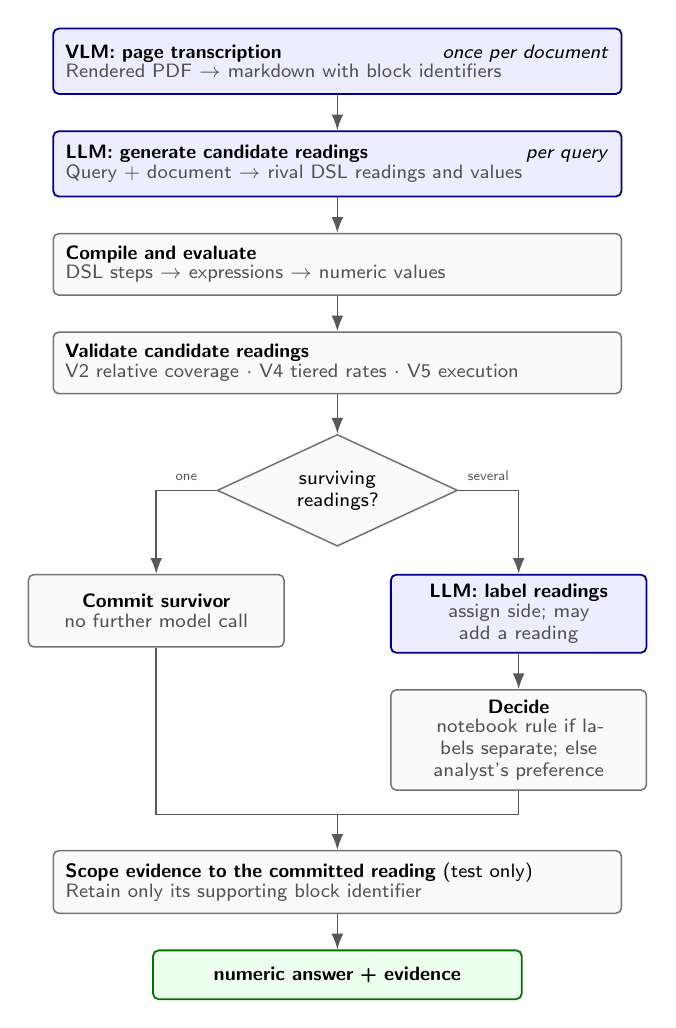
\begin{tikzpicture}[
  font=\sffamily\scriptsize,
  >=Latex,
  flow/.style={-{Latex[length=2mm]}, line width=0.55pt, draw=black!65},
  model/.style={
    draw=blue!55!black, fill=blue!7, line width=0.65pt,
    rounded corners=2pt, align=left, inner sep=4.5pt,
    text width=6.9cm, minimum height=0.83cm
  },
  rule/.style={
    draw=black!55, fill=black!2, line width=0.55pt,
    rounded corners=2pt, align=left, inner sep=4.5pt,
    text width=6.9cm, minimum height=0.78cm
  },
  branchmodel/.style={
    model, text width=3.0cm, minimum height=0.92cm,
    align=center, inner sep=3.5pt
  },
  branchrule/.style={
    rule, text width=3.0cm, minimum height=0.92cm,
    align=center, inner sep=3.5pt
  },
  decision/.style={
    diamond, aspect=2.15, draw=black!55, fill=black!2,
    line width=0.55pt, align=center, inner sep=1.5pt,
    text width=1.65cm
  },
  output/.style={
    draw=green!45!black, fill=green!7, line width=0.65pt,
    rounded corners=2pt, align=center, inner sep=4pt,
    text width=4.4cm, minimum height=0.62cm
  },
  note/.style={font=\sffamily\tiny, text=black!65, align=center}
]

\node[model] (vlm) {%
  \textbf{VLM: page transcription}\hfill\textit{once per document}\\[-1pt]
  \color{black!68}Rendered PDF $\rightarrow$ markdown with block identifiers};

\node[model, below=4.5mm of vlm] (analyst) {%
  \textbf{LLM: generate candidate readings}\hfill\textit{per query}\\[-1pt]
  \color{black!68}Query + document $\rightarrow$ rival DSL readings and values};

\node[rule, below=4.5mm of analyst] (compile) {%
  \textbf{Compile and evaluate}\\[-1pt]
  \color{black!68}DSL steps $\rightarrow$ expressions $\rightarrow$ numeric values};

\node[rule, below=4.5mm of compile] (validate) {%
  \textbf{Validate candidate readings}\\[-1pt]
  \color{black!68}V2 relative coverage $\cdot$ V4 tiered rates $\cdot$ V5 execution};

\node[decision, below=5mm of validate] (decision) {surviving\\readings?};

\node[branchrule, below left=7mm and -1mm of decision] (commit) {%
  \textbf{Commit survivor}\\[-1pt]
  \color{black!68}no further model call};

\node[branchmodel, below right=7mm and -1mm of decision] (review) {%
  \textbf{LLM: label readings}\\[-1pt]
  \color{black!68}assign side; may add a reading};

\node[branchrule, below=4.5mm of review] (close) {%
  \textbf{Decide}\\[-1pt]
  \color{black!68}notebook rule if labels separate; else analyst's preference};

% Merge the two branches below both boxes so the connector never crosses the
% text inside the lower ``Decide'' node.
\coordinate (merge) at ($(decision.south |- close.south)+(0,-3mm)$);

\node[rule, text width=6.9cm, below=4.5mm of merge] (scope) {%
  \textbf{Scope evidence to the committed reading} (test only)\\[-1pt]
  \color{black!68}Retain only its supporting block identifier};

\node[output, below=4.5mm of scope] (out) {\textbf{numeric answer + evidence}};

\draw[flow] (vlm) -- (analyst);
\draw[flow] (analyst) -- (compile);
\draw[flow] (compile) -- (validate);
\draw[flow] (validate) -- (decision);
\draw[flow] (decision.west) -| node[note, near start, above] {one} (commit.north);
\draw[flow] (decision.east) -| node[note, near start, above] {several} (review.north);
\draw[flow] (review) -- (close);
\draw[line width=0.55pt, draw=black!65] (commit.south) |- (merge);
\draw[line width=0.55pt, draw=black!65] (close.south) |- (merge);
\draw[flow] (merge) -- (scope);
\draw[flow] (scope) -- (out);

\end{tikzpicture}}
\caption{The \textsc{C3C} pipeline. Dark boxes are model calls (VLM, LLM);
white boxes are deterministic rules. When several readings survive and the labels do not separate
them, the analyst's preferred reading is kept. Evidence scoping (bottom) was
added for the test submission; the dev200 and replica arms use the task-level
evidence list.}
\label{fig:pipeline}
\end{figure}

\subsection{Adapting to the test regime}
\label{sec:submitted}

\paragraph{Submitted system.} During the competition we submitted \textsc{C3C}
on DeepSeek-V4-Flash, followed by a cascade of corrections that uses open
models only. The first step was deterministic post-processing: evidence was
scoped to the committed reading, the block parser was adapted to test
separators, and decimals were formatted. A targeted re-run then used a prompt
that told the model to locate the block containing the query's words; its
answer was adopted in 30 tasks. Next, in the manner of a model cascade \citep{chen2023frugalgpt}, Nemotron-3-Ultra \citep{nvidia2026nemotron3ultra} re-solved 270
low-confidence tasks with the \textsc{C3} prompt, and a DeepSeek-V4-Flash call
that saw both derivations adjudicated each disagreement. Last, DeepSeek-R1 \citep{deepseek2025r1} received the whole document for tasks whose cited block posed no question.
Appendix~\ref{app:submitted} gives the three attempts and the confidence
criterion. The targeted prompt was written after inspecting unlabelled test
documents, and its keyword rule is the heuristic that the decoys defeat
(\S\ref{sec:data}). Only the first attempt's portal score was visible during
the competition, and no stage was chosen by comparing portal scores.

\paragraph{Selection card.} After the competition we added one paragraph to
the \textsc{C3} prompt. It describes the decoy template and asks the model to
match the query to what a problem is about, not to repeated words (Appendix
\ref{app:prompts}). \textbf{It was written by inspecting test documents after
the deadline and was never part of a submitted system.} We apply it to
\textsc{C3} rather than \textsc{C3C} because the reviewer had no measurable
effect on the replica (\S\ref{sec:results}).

\section{Experimental setup}
\label{sec:setup}

\paragraph{Models and settings.} We called all models through OpenRouter\footnote{\url{https://openrouter.ai}; model names follow its
identifiers.}. The main model is DeepSeek-V4-Flash \citep{deepseek2026v4}, an
open-weight model. In the exploration phase it
was among the cheapest, and with \textsc{C3} it placed the gold value among
its readings in more hard-18 tasks than five other open models
(Appendix~\ref{app:sweep}). After the competition we added GLM-5.3-Flash \citep{glm2026glm5}, also
open-weight, for the replica. In all we ran 14 open-weight models;
Appendix~\ref{app:sweep} lists them and why only these two reached the main
results. All calls use temperature 1.0 with API
reasoning enabled. The analyst calls of \textsc{C2} and \textsc{C3} use high
effort and a 24{,}576-token ceiling, raised from 8{,}192 when test documents
exhausted it. The reviewer uses medium effort. Each variant run with a given model is an \emph{arm}. Every arm takes one sample per task; only the
final validation submission used self-consistency ($N{=}5$,
\citealp{wang2023selfconsistency}).

\paragraph{Costs.} In API fees, \textsc{A0} cost US\$0.07 and \textsc{C2}
US\$0.18 on dev200. Each replica arm cost between US\$0.10 and US\$2, with
\textsc{C3} on DeepSeek at US\$0.62. The test run of \textsc{C3C} cost about
US\$3--4, and each stage of the correction cascade cost under US\$4. Stage~1
ran locally on one RTX 3090. The closed agent ran under a subscription, so we
cannot report a comparable cost for it.

\paragraph{Closed references.} Our main reference is Claude
Code\footnote{\url{https://claude.com/claude-code}} with Claude Sonnet~5 \citep{anthropic2026sonnet5}
(medium effort), run on the replica in an isolated directory with the task
specification, the replica documents and the training data, which is what a
participant had. We scored its output outside that directory. Appendix
\ref{app:agent} gives the protocol and a possible leak of training answers. On hard-18 we also ran two closed models
inside our harness, GPT-5.6 Sol and Claude Fable 5.1 \citep{anthropic2026fable51}.

\paragraph{Statistics.} We report 95\% Wilson intervals \citep{wilson1927} and exact McNemar tests \citep{mcnemar1947}
on paired items, over the items both arms completed. For a pair of arms,
``$a$:$b$'' counts the items only the first arm or only the second arm gets
right. We do not correct for multiple comparisons. Where a result would not
survive a Bonferroni correction \citep{dunn1961} over the 16 replica tests in
Appendix~\ref{app:pvalues} (threshold $p\approx0.003$), we say so.

\section{Results}
\label{sec:results}

\subsection{Exploration phase}

\begin{table}[t]
\centering
\small
\setlength{\tabcolsep}{4pt}
\begin{tabularx}{\columnwidth}{>{\raggedright\arraybackslash}Xccc}
\toprule
arm & hard-18 & dev200 & val \\
& EM & EM & ans.\ / joint \\
\midrule
\textsc{A0}   & 0/18$^\ast$ & 167/200 & --- \\
\textsc{C2}   & 1/18$^\ast$ & 173/200 & --- \\
\textsc{C3}   & 3/18 & 163/200 & --- \\
\textsc{C3C}  & \textbf{7/18} & 165/200 & 88.48 / 88.02 \\
\textsc{C3C}+E/D & 7/18$^\S$ & \textbf{176/200}$^\S$ & \textbf{89.86} / \textbf{89.86}$^\dagger$ \\
\midrule
\textsc{C2} (Sol) & 2/18$^\ast$ & 165/200 & --- \\
\textsc{A0}/\textsc{C2} (Fable) & 1/16 / 1/16 & --- & --- \\
\bottomrule
\end{tabularx}
\caption{Exploration phase, using DeepSeek-V4-Flash unless a model is shown in
parentheses. E/D adds escalation and deliberation; Sol is GPT-5.6 Sol, and
Fable is Claude Fable 5.1. $^\ast$The 16 shared failures were selected as tasks
that \textsc{A0}, \textsc{C2}, and Sol all missed, so these arms can score only
on the two diagnostic cases; Fable ran only on the 16. For \textsc{C3},
dev200 counts the compiled answer; with the fallback to the model's stated
answer it scores 165. The val score of \textsc{C3C} uses one sample per task.
$^\dagger$With self-consistency ($N{=}5$) and a separate evidence call.
$^\S$Escalation and the separate evidence call only (one sample, no
deliberation); the escalation criterion was chosen on dev200. In the same run,
\textsc{C3C} recovers 5 of the hard-18 tasks.}
\label{tab:explore}
\end{table}

Table~\ref{tab:explore} summarises the exploration phase. On hard-18,
\textsc{C3} recovers 3 and \textsc{C3C} 7 of the 18 baseline failures.
\textsc{C2} and Sol cannot be compared on this set, because it was selected
from their failures. Fable, which played no part in the selection, recovered 1
of the 16. The set measures recovery, not accuracy, and the notebook's rules
were written while studying these cases, so the 7 is optimistic. Across six
open models, \textsc{C3} placed the gold value among its readings more often
than \textsc{C2} in four (Appendix~\ref{app:sweep}).

The dev200 set is not selected by difficulty, although it guided development.
On it, the differences between variants are small. Direct prompting is already at
83.5\%. \textsc{C2} gains six tasks overall; on the 198 items both arms
completed, it recovers 10 and loses 3 ($p=0.09$). \textsc{C3} falls ten tasks
below \textsc{C2} (3:11 on the 194 items both arms completed, $p=0.057$), and the notebook changes
6 tasks without a significant net effect (4:2, $p=0.69$). Escalating the tasks
flagged as low-confidence to Nemotron-3-Ultra, with a separate evidence call,
raises dev200 to 176 (11:0, $p=0.001$), although the flagging criterion was
chosen on the same set. On val, which has
one candidate passage per document, the pipeline reached 88.5--89.9\%. At the
end of the exploration phase, the structure appeared sound and the remaining
errors appeared to be rare interpretive cases.

\subsection{Test-regime phase}

\begin{table}[t]
\centering
\small
\setlength{\tabcolsep}{4pt}
\begin{tabular}{llrrr}
\toprule
model & arm & answer & evid. & joint \\
\midrule
DeepSeek & \textsc{A0}      & 46.3 & 46.0 & 40.3 \\
         & \textsc{C2}      & 53.0 & 60.3 & 50.7 \\
         & \textsc{C3}      & 49.3 & 46.0 & 38.7 \\
         & \textsc{C3}+card & 68.3 & 76.0 & 63.7 \\
\midrule
GLM      & \textsc{A0}      & 64.4 & 70.8 & 63.1 \\
         & \textsc{C2}      & 68.9 & 58.5 & 53.2 \\
         & \textsc{C3}      & 62.0 & 63.0 & 51.7 \\
         & \textsc{C3}+card & \textbf{77.7} & \textbf{80.3} & \textbf{67.0} \\
\midrule
\multicolumn{2}{l}{Claude Code (Sonnet 5)} & 82.0 & 94.0 & 82.0 \\
\bottomrule
\end{tabular}
\caption{Replica, \% over the items each arm completed: 300, except 295 for
\textsc{A0} GLM and 299 for \textsc{C2} GLM. For \textsc{C2} DeepSeek, 26 tasks that hit a provider rate
limit were rerun with the same configuration on another fp8 provider.
95\% intervals are $\pm$5--6 points. All replica runs took place after the
competition.}
\label{tab:replica}
\end{table}

Table~\ref{tab:replica} reports all variants on the replica, where selection matters.
Paired tests are in Appendix~\ref{app:pvalues}. We make four observations.
\begin{enumerate}
\item Against the baseline, the final configuration, which includes the
      post-deadline card, adds 22.0 answer points on DeepSeek and 13.3 on GLM
      (82:16 and 59:17, both $p<10^{-5}$).
\item \textsc{C2} raises answer accuracy over \textsc{A0} by 6.7 and 4.5
      points ($p=0.024$ and $0.036$), which would not survive a Bonferroni
      correction. On GLM it lowers joint accuracy (29:56, $p=0.005$), because
      rival readings that cited different blocks were submitted as a union.
      \textsc{C3} does not improve on \textsc{C2} in any of the four
      comparisons and is significantly worse in two. The notebook leaves
      DeepSeek unchanged (147 against 148 correct answers).
\item The selection card gives the largest single gain, +19.0 and +15.7
      points over \textsc{C3} ($p<10^{-7}$).
\item The model matters about as much as the technique. GLM prompted directly
      outperforms DeepSeek with \textsc{C3} (61:16, $p=2{\times}10^{-7}$).
\end{enumerate}

\begin{table}[t]
\centering
\small
\begin{tabular}{lrr}
\toprule
submission & answer & joint \\
\midrule
test, attempt 1 (\textsc{C3C})       & 51.4 & 34.6 \\
test, ranked (\textsc{C3C} + cascade) & --- & \textbf{45.09} \\
test, best team                       & --- & 85.09 \\
\midrule
val, \textsc{C3} GLM$^\S$        & 88.94 & 74.65 \\
val, \textsc{C3}+card GLM$^\S$   & 89.40 & 88.94 \\
\bottomrule
\end{tabular}
\caption{Portal scores. The final standings publish joint accuracy only.
$^\S$After the competition.}
\label{tab:official}
\end{table}

On the real test (Table~\ref{tab:official}), the answer accuracy of the
submitted \textsc{C3C} fell from 88.5\% on val to 51.4\% on test, with one
sample per task in both. The correction cascade raised
joint accuracy to 45.09\%, tied with two other teams for places 137--139 of
163. We cannot isolate the contribution of each stage. Evidence scoping is a
plausible main contributor, since the post-processing step cut multi-block
citations from 455 to 66. On val, the card leaves the answer unchanged but
improves citation (+14.3 joint).

\section{Discussion}
\label{sec:discussion}

\paragraph{Selection, not resolution.} We decomposed the errors of
\textsc{C3C} on the replica ($n=300$). Its answer accuracy there is 2.4 points
below the real test (49.0 against 51.4), and its joint accuracy is 4.1 points
above (38.7 against 34.6). Selection
errors, in which the cited block is not the target, make up 54.0\%
[48.3, 59.6]. In 31 of these 162 tasks the answer was nevertheless right.
Resolution errors, in which the target block is cited but the number is wrong,
make up 7.3\% [4.9, 10.9]. A decoy is the cited block in 88 of the 162
selection errors. Validators, the DSL and the notebook were designed for resolution. If they
leave the choice of passage unchanged, they can correct at most these 7.3\% of
tasks; this assumption is only approximate, since the variants also change
which blocks are cited (Table~\ref{tab:replica}). The card was designed for
selection, and it is the only component whose gain exceeds that bound.

\paragraph{Where the structure decides.} We recorded which path of
Figure~\ref{fig:pipeline} produced each \textsc{C3C} answer. On dev200, the
validators left a single surviving reading in 69 of 200 tasks and the
notebook closed 10. In 115 the analyst's preferred surviving reading was kept,
and 6 took a fallback path. On the replica, the validators decided 6 of 300
tasks and the notebook 17, while the analyst's own preference decided 274,
and 3 took a fallback path. Part of the validators' drop is mechanical:
\textsc{V2} and \textsc{V4} read the evidence text through the \texttt{bNN}
block format, so on documents with opaque identifiers only \textsc{V5} can
reject a reading.
The structure constrains and records the model's reasoning, but on the test
regime the final choice is almost always the model's own.

\paragraph{What the DSL adds.} The step-level DSL did not improve accuracy
over rival readings, but it changes what can be checked. The answer is the
compiled value of the committed steps, so the trace is faithful to the
computation that produced it, as in faithful chain-of-thought prompting
\citep{lyu2023faithful}, although not necessarily to how the model arrived at
the reading. Each \texttt{obs} step names a number taken from the passage and
each \texttt{assume} step states the interpretation applied to it, so a reader
or a rule can see which quantity was used and under which assumption. We used
this twice. Evidence scoping in the submitted system keeps a single block when
the committed reading's steps name it or observe numbers found only in it
(Appendix~\ref{app:submitted}), which cut multi-block citations from 455 to 66;
and the notebook rules act on labels given to the stated assumptions, not on
final numbers. We did not evaluate the traces with human readers.

\paragraph{Model-played antagonists.} Early versions of \textsc{C3C} also had
a panel of three jurors and an adversarial advisor, played by the analyst's own
model, to challenge the committed reading.
Across replays on hard-18, including runs in which a correct reading had been
injected into the candidates, the jury decided 19 cases and matched gold in
none, often unanimously. Replacing the jurors' model family (DeepSeek with Kimi; \citealp{kimi2025k2}) left 7 of 9 verdicts identical, with no dissent. The advisor was never
the sole cause of a correction, and we removed both before any test
submission. This agrees with reports that models do not reliably correct their
own reasoning without external feedback \citep{huang2024selfcorrect}, that
multi-agent debate often does not outperform simpler prompting
\citep{smit2024mad}, and with the premise of debate that the truth prevails when some participant
argues for it \citep{irving2018debate}. Instances that
share a reading prior appear to agree on the same wrong reading. With 19
decisions, all from hard-18, this observation is exploratory. In our setting, the components that changed outcomes either did
not involve the model (validators, compiled arithmetic, fixed rules) or used it
only to label or propose readings that a rule then evaluated. The deliberation
step of the submitted cascade is a different case, since it compares
derivations from two different models, but its effect on test could not be
isolated.

\paragraph{Model substitution.} Replacing DeepSeek entirely with
Nemotron-3-Ultra or DeepSeek-R1 repaired part of a subset of 35
known failures. On the full dev200, none was distinguishable from the
incumbent (paired $p\geq0.48$), because each fixed some tasks and broke others, the regression pattern known as negative flips \citep{yan2021pct}.

\paragraph{Comparison with a closed agent.} Claude Code reached 82.0\% on the
replica. On answers it is 4.3 points above our best open configuration, a
difference that is not significant (27:14, $p=0.06$). On joint accuracy it is
15.0 points above (58:13, $p=6{\times}10^{-8}$), mostly through evidence
(94.0\% against 80.3\%). Its notes show that it wrote a document parser,
learned the decoy template and settled the hardest selections itself; we addressed selection only after the competition, through the card. On answer accuracy, the gap between
GLM and this reference shrinks from 17.6 points with direct prompting to 4.3
with \textsc{C3} and the card; on joint accuracy, 15.0 points remain.

\section{Related work}

\textsc{C2} and \textsc{C3} belong to the program-aided family
\citep{gao2023pal,chen2023pot,ye2023satlm}, which moves the arithmetic of
chain-of-thought prompting \citep{wei2022cot} into executed code;
Section~\ref{sec:discussion} discusses why its benefit was small on the test
regime. DocSEM combines question answering over document images
\citep{mathew2021docvqa} with numerical reasoning over documents
\citep{chen2021finqa}. Separating citation from correctness follows ALCE
\citep{gao2023alce}. The selection problem resembles the distractor setting of
HotpotQA \citep{yang2018hotpotqa} and long-context distractor effects
\citep{liu2024lost}, and adding irrelevant or seemingly relevant statements to
grade-school math problems is known to lower accuracy
\citep{shi2023distracted,mirzadeh2025gsmsymbolic}. DocSEM's distractors,
however, are complete, solvable problems built to match the query's words
better than the target does. Even test sets rebuilt to the original
specification can lower accuracy \citep{recht2019imagenet}; in DocSEM, the
specification itself changes between validation and test. On
self-verification and debate, see \S\ref{sec:discussion}.

\section{Conclusion}

Without any training, inference-time structure improved two frozen open models
on a replica of the more complex held-out test regime. We draw four
conclusions. First, guidance helps most when it targets where the errors are:
most of the gain came from one paragraph on passage selection added after the
competition, not from the reasoning structure. Second, structure makes the
reasoning inspectable but not necessarily better: the step-level DSL did not
improve accuracy over rival readings, the model's own preference still decided
most answers on the test regime (\S\ref{sec:discussion}), and whether the
trace helps human readers remains untested. Third, copies of one model were
not independent reviewers: in an exploratory test, jurors played by the
analyst's own model agreed on the same wrong reading. Fourth, the model
matters about as much as the technique: a stronger model prompted directly
outperformed a weaker one with the step-level structure. The resulting systems
remained far from the top of the leaderboard. Two lessons from this participation may
be useful elsewhere. Comparing each variant with the previous one, and not
only with the baseline, is what exposed the DSL's null effect. Measuring the
input distribution of the test split before tuning would likely have revealed
the change of task before our submission.

\section*{Limitations}

All results come from one benchmark, whose problems are variants of
grade-school math problems that may overlap with the models' pretraining data.
The replica and every experiment on it were built and run after the
competition. The replica is synthetic and somewhat easier than test, and its agreement with the real test rests on a single comparison, with our first test submission. Of its 300
targets, 65 come from dev200 and 5 from hard-18, so it is not independent of
development. The selection card was derived from test documents after the
deadline, and the targeted re-run prompt of the submitted system was informed
by unlabelled test documents. The hard-18 set is selected from failures and
informed the notebook's rules, so it overstates the notebook's effect. The
dev200 set guided development and is not held out. We did not evaluate the
readability of derivations with human readers. The closed-agent comparison is
not controlled. The agent ran once, interactively, with code execution. It had
access to the published answers of the training problems embedded in the
replica and reports not having opened them. It settled 17 cases itself and, by
its own report, used an outcome record as the answer in 5, which our arms
never do. All arms are single runs, 26 \textsc{C2} DeepSeek tasks on the
replica were served by a different fp8 provider after a rate limit, and we do
not correct for multiple comparisons. The
correction cascade was never run on the replica, and the portal withheld one
attempt's score, so the 34.6$\rightarrow$45.09 gain cannot be attributed to a
single stage.

\section*{Acknowledgments}

We thank the DocInsights 2026 organisers for the task and the evaluation
infrastructure.

\begin{thebibliography}{}

\bibitem[Anthropic(2026a)]{anthropic2026sonnet5}
Anthropic. 2026a.
\newblock System card: {Claude Sonnet 5}.
\newblock \url{https://www.anthropic.com/claude-sonnet-5-system-card}. Accessed 2026-09-27.

\bibitem[Anthropic(2026b)]{anthropic2026fable51}
Anthropic. 2026b.
\newblock Introducing {Claude Fable 5.1} and {Claude Mythos 5.1}.
\newblock \url{https://www.anthropic.com/claude-fable-and-mythos-5-1}. Accessed 2026-09-27.

\bibitem[Auer et al.(2024)]{auer2024docling}
Christoph Auer, Maksym Lysak, Ahmed Nassar, et al. 2024.
\newblock Docling technical report.
\newblock arXiv:2408.09869.

\bibitem[Chen et al.(2021)]{chen2021finqa}
Zhiyu Chen, Wenhu Chen, Charese Smiley, Sameena Shah, Iana Borova, Dylan
  Langdon, Reema Moussa, Matt Beane, Ting-Hao Huang, Bryan Routledge, and
  William~Yang Wang. 2021.
\newblock {FinQA}: A dataset of numerical reasoning over financial data.
\newblock In {\em EMNLP}.

\bibitem[Chen et al.(2023)]{chen2023pot}
Wenhu Chen, Xueguang Ma, Xinyi Wang, and William W. Cohen. 2023.
\newblock Program of thoughts prompting: Disentangling computation from
  reasoning for numerical reasoning tasks.
\newblock {\em TMLR}. arXiv:2211.12588.

\bibitem[Chen et al.(2024)]{chen2023frugalgpt}
Lingjiao Chen, Matei Zaharia, and James Zou. 2024.
\newblock {FrugalGPT}: How to use large language models while reducing cost
  and improving performance.
\newblock {\em TMLR}. arXiv:2305.05176.

\bibitem[Cobbe et al.(2021)]{cobbe2021gsm8k}
Karl Cobbe, Vineet Kosaraju, Mohammad Bavarian, Mark Chen, Heewoo Jun, Lukasz
  Kaiser, Matthias Plappert, Jerry Tworek, Jacob Hilton, Reiichiro Nakano,
  Christopher Hesse, and John Schulman. 2021.
\newblock Training verifiers to solve math word problems.
\newblock arXiv:2110.14168.

\bibitem[DeepSeek-AI(2025)]{deepseek2025r1}
DeepSeek-AI. 2025.
\newblock {DeepSeek-R1}: Incentivizing reasoning capability in {LLMs} via
  reinforcement learning.
\newblock arXiv:2501.12948.

\bibitem[DeepSeek-AI(2026)]{deepseek2026v4}
DeepSeek-AI. 2026.
\newblock {DeepSeek-V4}: Towards highly efficient million-token context
  intelligence.
\newblock arXiv:2606.19348.

\bibitem[Dunn(1961)]{dunn1961}
Olive Jean Dunn. 1961.
\newblock Multiple comparisons among means.
\newblock {\em Journal of the American Statistical Association},
  56(293):52--64.

\bibitem[Freedman et al.(2025)]{freedman2025argllm}
Gabriel Freedman, Adam Dejl, Deniz Gorur, Xiang Yin, Antonio Rago, and
  Francesca Toni. 2025.
\newblock Argumentative large language models for explainable and contestable
  claim verification.
\newblock In {\em AAAI}. arXiv:2405.02079.

\bibitem[Gao et al.(2023a)]{gao2023pal}
Luyu Gao, Aman Madaan, Shuyan Zhou, Uri Alon, Pengfei Liu, Yiming Yang, Jamie
  Callan, and Graham Neubig. 2023.
\newblock {PAL}: Program-aided language models.
\newblock In {\em ICML}. arXiv:2211.10435.

\bibitem[Gao et al.(2023b)]{gao2023alce}
Tianyu Gao, Howard Yen, Jiatong Yu, and Danqi Chen. 2023.
\newblock Enabling large language models to generate text with citations.
\newblock In {\em EMNLP}. arXiv:2305.14627.

\bibitem[GLM-5 Team(2026)]{glm2026glm5}
GLM-5 Team. 2026.
\newblock {GLM-5}: From vibe coding to agentic engineering.
\newblock arXiv:2602.15763.

\bibitem[Gururangan et al.(2018)]{gururangan2018annotation}
Suchin Gururangan, Swabha Swayamdipta, Omer Levy, Roy Schwartz, Samuel~R. Bowman,
  and Noah~A. Smith. 2018.
\newblock Annotation artifacts in natural language inference data.
\newblock In {\em NAACL}.

\bibitem[Hu et al.(2022)]{hu2022lora}
Edward~J. Hu, Yelong Shen, Phillip Wallis, Zeyuan Allen-Zhu, Yuanzhi Li, Shean
  Wang, Lu~Wang, and Weizhu Chen. 2022.
\newblock {LoRA}: Low-rank adaptation of large language models.
\newblock In {\em ICLR}. arXiv:2106.09685.

\bibitem[Huang et al.(2024)]{huang2024selfcorrect}
Jie Huang, Xinyun Chen, Swaroop Mishra, Huaixiu Steven Zheng, Adams Wei Yu,
  Xinying Song, and Denny Zhou. 2024.
\newblock Large language models cannot self-correct reasoning yet.
\newblock In {\em ICLR}. arXiv:2310.01798.

\bibitem[Irving et al.(2018)]{irving2018debate}
Geoffrey Irving, Paul Christiano, and Dario Amodei. 2018.
\newblock AI safety via debate.
\newblock arXiv:1805.00899.

\bibitem[Kimi Team(2025)]{kimi2025k2}
Kimi Team. 2025.
\newblock {Kimi K2}: Open agentic intelligence.
\newblock arXiv:2507.20534.

\bibitem[Liu et al.(2024)]{liu2024lost}
Nelson F. Liu, Kevin Lin, John Hewitt, Ashwin Paranjape, Michele Bevilacqua,
  Fabio Petroni, and Percy Liang. 2024.
\newblock Lost in the middle: How language models use long contexts.
\newblock {\em TACL}.

\bibitem[Lyu et al.(2023)]{lyu2023faithful}
Qing Lyu, Shreya Havaldar, Adam Stein, Li Zhang, Delip Rao, Eric Wong,
  Marianna Apidianaki, and Chris Callison-Burch. 2023.
\newblock Faithful chain-of-thought reasoning.
\newblock In {\em IJCNLP-AACL}. arXiv:2301.13379.

\bibitem[Mathew et al.(2021)]{mathew2021docvqa}
Minesh Mathew, Dimosthenis Karatzas, and C.~V. Jawahar. 2021.
\newblock {DocVQA}: A dataset for {VQA} on document images.
\newblock In {\em WACV}.

\bibitem[McNemar(1947)]{mcnemar1947}
Quinn McNemar. 1947.
\newblock Note on the sampling error of the difference between correlated
  proportions or percentages.
\newblock {\em Psychometrika}, 12(2):153--157.

\bibitem[Mirzadeh et al.(2025)]{mirzadeh2025gsmsymbolic}
Iman Mirzadeh, Keivan Alizadeh-Vahid, Hooman Shahrokhi, Oncel Tuzel, Samy Bengio, and
  Mehrdad Farajtabar. 2025.
\newblock {GSM-Symbolic}: Understanding the limitations of mathematical
  reasoning in large language models.
\newblock In {\em ICLR}. arXiv:2410.05229.

\bibitem[Niu et al.(2025)]{niu2025mineru25}
Junbo Niu, Zheng Liu, Zhuangcheng Gu, et al. 2025.
\newblock {MinerU2.5}: A decoupled vision-language model for efficient
  high-resolution document parsing.
\newblock arXiv:2509.22186.

\bibitem[NVIDIA(2026)]{nvidia2026nemotron3ultra}
NVIDIA. 2026.
\newblock {Nemotron 3 Ultra}: Open, efficient mixture-of-experts hybrid
  {Mamba-Transformer} model for agentic reasoning.
\newblock arXiv:2606.15007.

\bibitem[OpenAI(2026)]{openai2026gpt56}
OpenAI. 2026.
\newblock {GPT-5.6} system card.
\newblock \url{https://deploymentsafety.openai.com/gpt-5-6}. Accessed 2026-09-27.

\bibitem[Poznanski et al.(2025)]{poznanski2025olmocr2}
Jake Poznanski, Luca Soldaini, and Kyle Lo. 2025.
\newblock {olmOCR} 2: Unit test rewards for document {OCR}.
\newblock arXiv:2510.19817.

\bibitem[Recht et al.(2019)]{recht2019imagenet}
Benjamin Recht, Rebecca Roelofs, Ludwig Schmidt, and Vaishaal Shankar. 2019.
\newblock Do {ImageNet} classifiers generalize to {ImageNet}?
\newblock In {\em ICML}.

\bibitem[Shi et al.(2023)]{shi2023distracted}
Freda Shi, Xinyun Chen, Kanishka Misra, Nathan Scales, David Dohan, Ed~H. Chi,
  Nathanael Sch{\"a}rli, and Denny Zhou. 2023.
\newblock Large language models can be easily distracted by irrelevant
  context.
\newblock In {\em ICML}. arXiv:2302.00093.

\bibitem[Singh et al.(2026)]{singh2026gsmsem}
Jyotika Singh, Fang Tu, Aziza Mirsaidova, Amit Agarwal, Hitesh Laxmichand
  Patel, Sandip Ghoshal, Miguel Ballesteros, Karan Dua, Yassine Benajiba,
  Weiyi Sun, Tao Sheng, Graham Horwood, Sujith Ravi, and Dan Roth. 2026.
\newblock {GSM-SEM}: Benchmark and framework for generating semantically
  variant augmentations.
\newblock arXiv:2605.07053.

\bibitem[Smit et al.(2024)]{smit2024mad}
Andries~P. Smit, Nathan Grinsztajn, Paul Duckworth, Thomas~D. Barrett, and
  Arnu Pretorius. 2024.
\newblock Should we be going {MAD}? {A} look at multi-agent debate strategies
  for {LLMs}.
\newblock In {\em ICML}. arXiv:2311.17371.

\bibitem[Wang et al.(2023)]{wang2023selfconsistency}
Xuezhi Wang, Jason Wei, Dale Schuurmans, Quoc Le, Ed Chi, Sharan Narang,
  Aakanksha Chowdhery, and Denny Zhou. 2023.
\newblock Self-consistency improves chain of thought reasoning in language
  models.
\newblock In {\em ICLR}.

\bibitem[Wei et al.(2022)]{wei2022cot}
Jason Wei, Xuezhi Wang, Dale Schuurmans, Maarten Bosma, Brian Ichter, Fei Xia,
  Ed~H. Chi, Quoc~V. Le, and Denny Zhou. 2022.
\newblock Chain-of-thought prompting elicits reasoning in large language
  models.
\newblock In {\em NeurIPS}.

\bibitem[Wilson(1927)]{wilson1927}
Edwin B. Wilson. 1927.
\newblock Probable inference, the law of succession, and statistical
  inference.
\newblock {\em Journal of the American Statistical Association},
  22(158):209--212.

\bibitem[Yan et al.(2021)]{yan2021pct}
Sijie Yan, Yuanjun Xiong, Kaustav Kundu, Shuo Yang, Siqi Deng, Meng Wang, Wei
  Xia, and Stefano Soatto. 2021.
\newblock Positive-congruent training: Towards regression-free model updates.
\newblock In {\em CVPR}.

\bibitem[Yang et al.(2018)]{yang2018hotpotqa}
Zhilin Yang, Peng Qi, Saizheng Zhang, Yoshua Bengio, William W. Cohen, Ruslan
  Salakhutdinov, and Christopher D. Manning. 2018.
\newblock {HotpotQA}: A dataset for diverse, explainable multi-hop question
  answering.
\newblock In {\em EMNLP}.

\bibitem[Ye et al.(2023)]{ye2023satlm}
Xi Ye, Qiaochu Chen, Isil Dillig, and Greg Durrett. 2023.
\newblock {SatLM}: Satisfiability-aided language models using declarative
  prompting.
\newblock In {\em NeurIPS}. arXiv:2305.09656.

\end{thebibliography}

\appendix
\section{Replica construction and validity gate}
\label{app:replica}

Each training target block is stripped of the training template's framing
sentence and embedded in a generated document. The document contains 22
competing question blocks from the remaining pool, a variable number of
decoys carrying the query's anchors, filler prose from non-target blocks,
opaque identifiers sampled from the eight shapes and three separators seen in
test, and ``outcome records'' for about 70\% of non-target cases and never for
the target. Queries follow the three observed templates. No withheld label is
reconstructed: the gold is known because we choose the target.

Two construction artefacts were caught by the gate before any model ran.
First, targets had kept a framing sentence listing the query anchors
verbatim. Second, decoys mentioned each anchor once while targets repeat their
vocabulary, so counting anchors found the target 60.6\% of the time against a
chance rate of 14.5\%. After both fixes, on $n=276$, keyword matching scores
27.9\% [22.9, 33.5], the longest candidate 30.1\%, the first candidate 29.7\%,
and random choice among candidates 29.6\%. These figures come from the
released implementation of the gate. The script used before the runs was not
preserved; it gave 23.4\% for keyword matching against 31.3\% for random
choice ($n=278$). The replica is easier than test:
it averages 36k against 43k characters per document, has a lighter tail of
anchor competitors, and has no decimal answers. Absolute scores on it are
therefore optimistic.

\section{Submitted system}
\label{app:submitted}

\begin{table}[h]
\centering
\small
\setlength{\tabcolsep}{3.5pt}
\begin{tabularx}{\columnwidth}{>{\raggedright\arraybackslash}Xrrrr}
\toprule
step & $\Delta$ans. & $\Delta$evid. & multi-block & joint \\
\midrule
attempt 1 (\textsc{C3C})          & ---  & ---  & 455 & 34.62 \\
+ post-proc.\ + targeted           & 189  & 453  &  66 & \\
+ escalation + deliberation        &  43  &   0  &  66 & \\
+ R1 fallback (attempt 2)          &  51  &  61  &  66 & withheld \\
+ evidence narrowing (attempt 3)   &   1  &  41  &  27 & \textbf{45.09} \\
\bottomrule
\end{tabularx}
\caption{The three test attempts. $\Delta$ counts tasks whose answer or
evidence changed at that step; gold evidence is always one block. The portal
ranks each team's best attempt and selected attempt 3.}
\label{tab:lineage}
\end{table}

Attempt 1 ran \textsc{C3C} on DeepSeek-V4-Flash with one sample per task.
Attempt 2 added four stages.
(i)~Deterministic post-processing: evidence scoped to the committed reading,
a block parser for the test separators, repair of unknown identifiers, and
decimal formatting. Scoping keeps a single block when the committed reading's
step text names exactly one candidate block, or when the numbers it observes
appear in exactly one candidate block; otherwise the list is left unchanged.
(ii)~A targeted \textsc{C3} re-run on the 113 tasks whose cited block lacked
the query's words. It was adopted in 30.
(iii)~Escalation. A task was flagged as low-confidence if the validators had
not decided it on their own, or if its reasoning trace exceeded the 88th
percentile of reasoning tokens. Both signals had predicted errors on dev200.
Nemotron-3-Ultra re-solved the 270 flagged tasks on the isolated block, and a
DeepSeek-V4-Flash call, shown both derivations anonymised, adopted the
escalated answer in 43.
(iv)~A benchmark-agnostic DeepSeek-R1 call over the whole document for the 155
tasks whose cited block posed no question. It resolved 152.
Attempt 3 narrowed multi-block evidence using R1's choice, but only within the
blocks already cited. The ranked file changes 272 answers and 506 evidence
lists relative to attempt 1.

\section{Paired tests on the replica}
\label{app:pvalues}

\begin{table}[h]
\centering
\scriptsize
\setlength{\tabcolsep}{2pt}
\begin{tabularx}{\columnwidth}{@{}l>{\raggedright\arraybackslash}Xrrrr@{}}
\toprule
& & \multicolumn{2}{c}{answer} & \multicolumn{2}{c}{joint} \\
model & comparison & $a$:$b$ & $p$ & $a$:$b$ & $p$ \\
\midrule
DeepSeek & \textsc{C2} vs \textsc{A0}   & 46:26 & .024 & 57:26 & $9{\times}10^{-4}$ \\
         & \textsc{C3} vs \textsc{C2}   & 28:39 & .22  & 25:61 & $1{\times}10^{-4}$ \\
         & card vs \textsc{C3}          & 73:16 & $7{\times}10^{-10}$ & 93:18 & $2{\times}10^{-13}$ \\
         & best vs \textsc{A0}          & 82:16 & $7{\times}10^{-12}$ & 91:21 & $1{\times}10^{-11}$ \\
\midrule
GLM      & \textsc{C2} vs \textsc{A0}   & 34:18 & .036 & 29:56 & .005 \\
         & \textsc{C3} vs \textsc{C2}   & 17:38 & .007 & 41:45 & .75 \\
         & card vs \textsc{C3}          & 61:14 & $4{\times}10^{-8}$ & 71:25 & $3{\times}10^{-6}$ \\
         & best vs \textsc{A0}          & 59:17 & $1{\times}10^{-6}$ & 52:38 & .17 \\
\bottomrule
\end{tabularx}
\caption{Each variant against the previous one; ``best'' is \textsc{C3}+card, also
compared with \textsc{A0}. $a$:$b$ counts items only the first or only the
second variant gets right. On GLM,
\textsc{C2} lowers joint accuracy because rival readings citing different
blocks submitted their union, the failure that evidence scoping later fixed.
The closed agent against the best open arm: answer 27:14 ($p=0.06$), joint
58:13 ($p=6{\times}10^{-8}$).}
\end{table}

\section{Models tested}
\label{app:sweep}

Table~\ref{tab:models} lists every model we ran and why only DeepSeek-V4-Flash
and GLM-5.3-Flash reached the main results. Each model is compared with
DeepSeek-V4-Flash on the same tasks and metric, given in the block heading;
$\Delta$ is the difference in percentage points. The counts behind the first
two blocks follow.

\begin{table*}[t]
\centering
\small
\setlength{\tabcolsep}{5pt}
\begin{tabularx}{\textwidth}{@{}lr>{\raggedright\arraybackslash}X@{}}
\toprule
model & $\Delta$ (pp) & why it was not used \\
\midrule
\multicolumn{3}{@{}l}{\emph{hard-18: gold value among the \textsc{C3} readings (DeepSeek-V4-Flash 44.4\%)}} \\
Kimi-K2.6        & $-5.6$  & Slightly lower coverage at 19$\times$ the cost, with 6 of 18 outputs unparsable. \\
Gemma-4-31B      & $-5.6$  & Slightly lower coverage, and the slowest model (median 136\,s per task). \\
Qwen3.8-Flash    & $-16.7$ & Lower coverage, and \textsc{C3} added nothing over \textsc{C2}. \\
MiniMax-M3       & $-27.8$ & Much lower coverage, and \textsc{C3} made it worse than \textsc{C2}. \\
DeepSeek-V4-Pro  & $-27.8$ & Much lower coverage despite being the larger DeepSeek model. \\
\midrule
\multicolumn{3}{@{}l}{\emph{26-task slice: exact answers with \textsc{C2} (DeepSeek-V4-Flash 38.5\%, fixed by the slice's construction)$^\ast$}} \\
Qwen3.8-Max      & $-26.9$ & 20 of 26 \textsc{C2} calls failed, at the highest cost of the slice. \\
Kimi-K2.7-Code   & $-11.5$ & Weakest direct-prompting baseline of the slice (2 of 26). \\
Laguna-S-2.1     & $-19.2$ & Lower with \textsc{C2} and weak under direct prompting. \\
Muse-Glimmer-30B & $-19.2$ & Same result as Laguna-S-2.1 at five times its cost. \\
\midrule
\multicolumn{3}{@{}l}{\emph{dev200: answer accuracy as the \textsc{C3C} analyst (DeepSeek-V4-Flash 82.5\%)}} \\
Nemotron-3-Ultra & $-3.0$  & Lower accuracy and frequent timeouts; kept only to re-solve low-confidence tasks. \\
DeepSeek-R1      & $-2.5$  & Lower accuracy at 10$\times$ the cost; kept only for the evidence call and the fallback. \\
MiMo-V2.5-Pro    & $0.0$   & Same accuracy at 4.6$\times$ the cost, with weaker evidence (192 against 196). \\
\midrule
\multicolumn{3}{@{}l}{\emph{Replica: answer accuracy with direct prompting (DeepSeek-V4-Flash 46.3\%)}} \\
GLM-5.3-Flash    & $+18.1$ & Kept as the second main model: the strongest open baseline on the replica. \\
Qwen3.7-Flash    & $-9.0$  & Lower baseline, and its weights are not open. \\
\midrule
\multicolumn{3}{@{}l}{\emph{Closed references, outside the open-model scope}} \\
GPT-5.6 Sol      & $-4.0$  & Closed; dev200 accuracy with \textsc{C2}, against 86.5\% for DeepSeek-V4-Flash. \\
Claude Fable 5.1 & ---     & Closed; run only on the 16 hard tasks, where DeepSeek-V4-Flash scores 0 by construction. \\
Claude Sonnet 5  & $+18.3$ & Closed agent (Claude Code); replica joint accuracy against 63.7\% for DeepSeek-V4-Flash with \textsc{C3}+card. \\
\bottomrule
\end{tabularx}
\caption{Models tested, compared with DeepSeek-V4-Flash on the same tasks.
All open models were called through OpenRouter. $^\ast$The slice holds 16
tasks DeepSeek-V4-Flash missed with both \textsc{A0} and \textsc{C2} and 10 it
solved only with \textsc{C2}, so the comparison favours it.}
\label{tab:models}
\end{table*}

On hard-18, the number of tasks whose gold value appears among the
arm's readings (whether or not it was the committed one) was, for \textsc{C2} and \textsc{C3} respectively: DeepSeek-V4-Flash 5 and 8,
Qwen3.8-Flash 5 and 5, Kimi-K2.6 4 and 7, Gemma-4-31B 4 and 7, MiniMax-M3 5
and 3, and DeepSeek-V4-Pro 1 and 3. On a 26-task slice (hard failures plus
tasks \textsc{C2} had newly solved, so biased toward \textsc{C2}), the
\textsc{A0}/\textsc{C2} counts were: Kimi-K2.6 7/3, Qwen3.8-Max 7/3,
Qwen3.8-Flash 7/4, Gemma-4-31B 6/7, MiniMax-M3 5/8, Kimi-K2.7-Code 2/7,
Laguna-S-2.1 4/5 and Muse-Glimmer-30B 4/5. On this biased slice, \textsc{C2}
scored above \textsc{A0} for the models weakest under direct prompting and
below it for the strongest.

\section{Selection card variants}
\label{app:card}

A second variant of the card adds that a case with a printed ``outcome
record'' is already resolved. On the replica this clause is true by
construction, so it is circular there. It scores 76.3\% (DeepSeek) and 78.7\%
(GLM), against 68.3\% and 77.7\% for the decoy-only card, inflating DeepSeek
by 8.0 points (42:18, $p=0.003$). We report only the decoy-only card.

\section{Closed-agent protocol}
\label{app:agent}

The agent (Claude Sonnet~5, medium effort) ran in a directory holding the task specification, the 300 replica
documents without labels, and the 908 training instances with gold. The
replica's targets are among those training problems, so a lookup was
possible in principle; the agent's notes state that it did not open the
training file. It was
told to write predictions and notes there and not to leave the directory. No
conclusion of this project was shown to it. It worked for about an hour. It
wrote a parser, excluded the decoy template by pattern, settled 17 ambiguous
selections itself, and delegated the arithmetic to subagents. By its own
report, it used a printed outcome record as the answer in 5 instances. Its
predictions were scored outside the directory against the replica's gold.

\section{Prompts}
\label{app:prompts}

We reproduce verbatim the three prompts on which the main results and
integrity statements depend: the \textsc{C3} analyst, the targeted re-run, and
the selection card. The \textsc{A0} and \textsc{C2} prompts, the \textsc{C3C}
reviewer, the deliberation prompt, and the DeepSeek-R1 fallback are available
in the released repository. The user message of every call holds the query and
the stage-1 markdown document.

\paragraph{\textsc{C3} analyst.} This prompt was used unchanged on dev200, on
the replica and in test attempt 1. Its schema still shows a \texttt{bNN}
evidence example inherited from train and val, although test identifiers are
opaque (\S\ref{sec:data}).
\begin{lstlisting}[style=prompt]
You solve a document-grounded quantitative question.

Rules:
- Use only the document in the user message. Do not use the filename, instance id, or outside knowledge.
- Do not combine facts from different passages unless the target scenario itself requires it.
- Do not recall or copy a similar GSM8K / textbook template.
- Do not invent block identifiers.

How to read the document:
- The document is in reading order.
- A line <<<PAGE n>>> marks a page break. A paragraph may be cut there; text at the top of the next page without a new label continues the previous block.
- Position comments such as <!-- bbox ... --> are not evidence ids.

Write a public derivation the runtime can compile, then execute. Emit TWO JSON objects, in this order.

1) State -- two rival readings:
{"evidence":["bNN"],"readings":[{"id":"r1","steps":[{"op":"obs","id":"a","value":0},{"op":"assume","text":"..."},{"op":"therefore","id":"q","expr":"a"},{"op":"return","expr":"q"}]},{"id":"r2","steps":[]}],"commit":"r1"}

- Exactly two readings. They must differ in the meaning of a number, quantifier, unit, or anaphor -- not in rounding.
- steps is an open list. Useful verbs: obs, assume, considering, therefore, isolate, return. Also fine: given, hence, deduce, let, if, then, compute, conclude. Unknown verbs still compile when they carry value or expr.
- obs (or take / read / bind) attaches a quantity from the evidence to an id.
- assume / considering / if / given states the warrant of that reading. It does not have to be arithmetic.
- therefore / hence / deduce / then writes arithmetic using bound ids and + - * / ( ).
- return names the expression that answers the query. The runtime compiles it; you may omit a top-level expression field.
- You may add extra steps (units, cases, business conditions, scientific caveats). Do not invent a closed schema of sides.
- Optional expression on the reading is a fallback if compile fails. Do not set result to 0 unless the answer is 0.
- commit is the reading you prefer.

2) Official prediction, and nothing after it:
{"instance_id":"<id>","answer":"<final number>","evidence":["bNN"]}

answer must match the committed compiled result. evidence must match state.evidence.
\end{lstlisting}

\paragraph{Targeted re-run (submitted, attempt 2).} Used on the 113 tasks
whose cited block lacked the query's words. It is the \textsc{C3} prompt with
the \texttt{bNN} examples replaced by ``\texttt{<block id, copied verbatim>}''
and the following block appended. Its first rule is the keyword heuristic that
the test decoys defeat (\S\ref{sec:data}). The Nemotron escalation used the
unmodified \textsc{C3} prompt.
\begin{lstlisting}[style=prompt]
TARGETING THE RIGHT BLOCK (this document holds many solvable sub-problems)

This document contains several complete, plausible quantitative problems -- most
of them are distractors. Exactly one answers the query. Before deriving anything:

- The query names its subject, e.g. "concerning X and Y". The target block
  contains those same words. Locate it first, then solve only that block.
- Blocks are labelled with an opaque identifier printed at the start of the
  line (for example `D#73:`, `RB2-5E9.`, `2032 `). Copy the identifier exactly
  as printed. Never normalise it, never renumber it, and never invent an id of
  the form b01/b02 -- that scheme does not exist in this document.
- `evidence` must list the block your COMMITTED reading actually used, and
  normally that is exactly one block. Do not list every block you looked at.
- If a block states a previously recorded outcome for a case, it is context,
  not the derivation: still cite the block that poses the question.
\end{lstlisting}

\paragraph{Selection card.} This paragraph is inserted into the \textsc{C3}
prompt after the reading instructions (decoy-only variant):
\begin{lstlisting}[style=prompt]
Selecting the target passage:
- The document contains many self-contained quantitative sub-problems. Only one
  answers the query. The others are complete, solvable problems that are not
  being asked about.
- The query names two lexical anchors. A block that repeats those anchors
  verbatim inside a counting template -- "In a separate concerning and X and Y
  record, <someone> counted (a + b) items in the first review and c in the
  second review" -- is a distractor. Its surface form matches the query more
  closely than the target does.
- Match the anchors to what the problem is ABOUT, not to literal repetition.
\end{lstlisting}

\end{document}
